\section{Work Flow}
There are three main sections to a CFD analysis: meshing, simulation, and analysis. DSMC-PIC is a subsection of CFD, therefore, the original developers have designed systems for all three sections, but most CFD analysis does not require the user to do all three tasks each time. A single mesh can produce many different simulations, and there can be many different analysis tasks from the same simulation. Therefore, SINATRA was broken down into three parts according to the three tasks it is able to accomplish. Each of those sections have their own repository, source code, and executables. They also share a resources repository between them. This allows the user to work in the meshing system and create the mesh or meshes necessary for their task. Then they move to the simulation system and use the newly created meshes as part of the simulation input. Once they have simulated the domain, they can take the created output files and run different analysis codes or create their own for their specific task.


% TO DO make sure that  cart3d has a 3d octree mesher
% TO DO - do I need trademark things here?

\begin{figure}
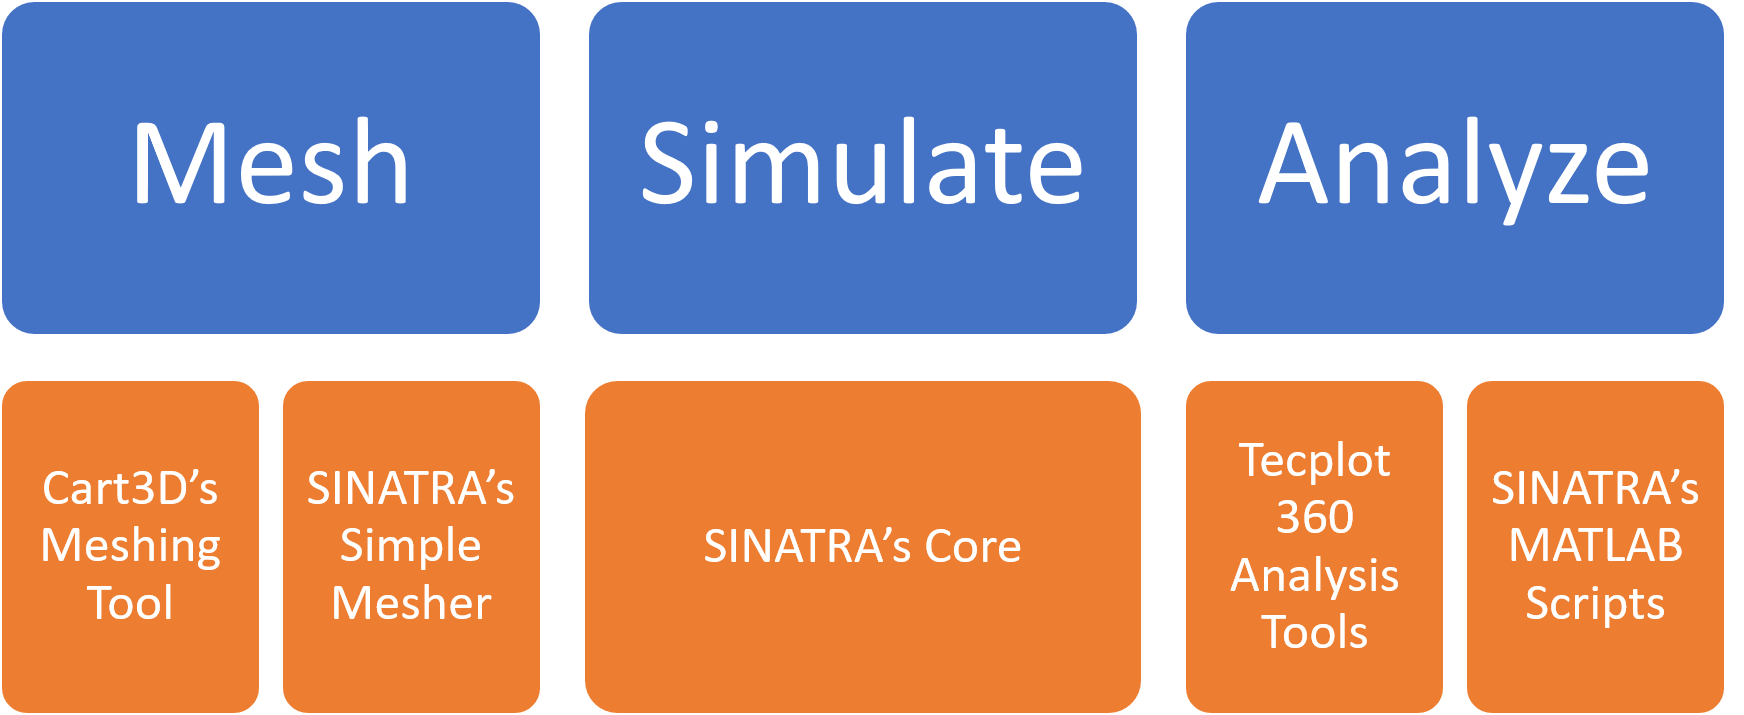
\includegraphics[width=.95\textwidth]{figures/UserWorkFlow.png}
\centering
\caption{Work flow System for SINATRA}
\label{fig:UserWorkFlow}
\end{figure}

\subsection{Mesh}
The original developers have designed this work flow for SINATRA while including the option for third party software to be used for the meshing and analysis sections. As seen in figure \ref{fig:UserWorkFlow}, Cart3D\textsuperscript{TM} \footnote{Cart3D Documentation - \url{http://www.nanda.org/}} was chosen to be the meshing 3rd party additional tool. Meshing a domain for SINATRA requires an Octree Mesh. For cases where the domain is empty, the homegrown SINATRA meshing tool is quick and simple; however, when an object is added to the domain, meshing becomes a much more complicated task (outside the scope and purpose of SINATRA).  Cart3D\textsuperscript{TM} is a CFD analysis tool by NASA which is available to universities. It has within it a three-dimensional octree meshing tool, which can take geometries and domain sizing as inputs. SINATRA will take the outputted mesh and use it for simulations. Cart3D has not been tested with SINATRA. It has been slated for future work for another developer to fully integrate Cart3D\textsuperscript{TM} and geometry boundaries with SINATRA\footnote{It may be necessary to run Cart3D within a Linux\textsuperscript{TM} virtual box for Windows\textsuperscript{TM} users}. \par

\subsection{Simulation}

SINATRA has been designed to be simple to develop and execute. Execution is completed through one executable file and one input text file. For simplicity, Windows\textsuperscript{TM} users can drag the .txt file onto the .exe file to run the simulation. SINATRA was deliberately built to be machine independent to reduce the risk of the code not being developed further or used for new tasks. The executable and output do not depend on using a specific Integrated Developer Environment like Visual Studio\textsuperscript{TM} or even using a certain operating system. A user can run many simulations or string together meshing, simulating, and analysis simply through a batch script. An example script is shown in Appendix \ref{app:examplescript}. \par
\indent Because SINATRA was built to be platform independent, it is very easy to compile. It requires only a single command with zero libraries\footnote{Need openmp for parallelization}. There are sample compile statements in the ReadME and compile scripts, but even an intermediate C++ coder could figure out how to compile SINATRA from the file list alone. This helps new developers move quickly through the code learning phase and can even allow beginners to explore the code base and test more complicated features. SINATRA has been tested through being compiled with various compilers and on different operating systems.

% TO DO add ppt graphic of this codeflow one with all the files and titles - appendix


\subsection{Analysis}
% Future make simple tecplot analysis script
% TO dO add citattions of david and macs thesies
% TO DO make analysis functions which gooes through all the cells (send anamynous function)


 After the simulation phase is completed, the user can use the SINATRA output files for analysis. The original developers created MATLAB scripts within SINATRA, which do basic types of analysis. For other analysis, Tecplot 360\textsuperscript{TM} \footnote{Tecplot 360 CFD post processing tools to analyzedata - \url{https://www.tecplot.com/products/tecplot-360/}} has been chosen as a third party tool. Tecplot\textsuperscript{TM} is a specific CFD analysis and visualization tool, which can show the mesh, geometry, and fluid flow. It includes robust visualization and animation tools as well as various analysis functions. SINATRA can output data in a format that Tecplot\textsuperscript{TM} reads natively. Tecplot\textsuperscript{TM} and SINATRA’s integration has been tested and used by the first developers.\par
 \indent SINATRA’s analysis section has not been built with an encompassing set of features to complete any task. It is up to the future users to determine the analysis they need to accomplish, edit SINATRA’s output class to accommodate, and compile the output data into the format they need. This can be completed through looking at SINATRA’s output class and reformatting other analysis techniques for the task at hand. Tecplot\textsuperscript{TM} and the included MATLAB scripts can do a majority of the beginning analysis, but the most detailed tools will need to be built by new developers.

 
\subsection{Execution Time}
A DSMC code is by nature a very computationally intense program. It requires a large amount of memory to store all of the data of each particle and mesh cell. It requires a lot of computational power to calculate the movement and collisions, therefore, it is important to design the code to be efficient and powerful. This is why C++ and classes were chosen for SINATRA; however, it is still a slow simulation for a large meshes with high particle densities. It is slated as future work for a developer who specializes in computer science and computational optimization to reduce the execution time of large SINATRA runs, but there are a few bottlenecks and available improvements which were added by the author. These help manage simulation time, especially when the Poisson equation solver is included. \par

\indent The simplest and most effective way to reduce simulation time on a DSMC simulation is parallelization. Parallelization is a complex and involved field with many competing ideas on best practices. There are many discussions about best ways to parallelize DSMC codes and PIC codes. Parallelization itself is also on the forefront of new technology in this age. Moore’s law has allowed programmers to have a large amount of memory for their simulation, so that is rarely the constricting factor. Processors seem to have become as powerful as they will be for user made systems on languages like C++\textsuperscript{TM}. Breaking the simulation between multiple cores or even within the GPU seems to be the new normal for decreasing execution times. For SINATRA, there are many parallelization possibilities. It is slated for future work for another developer to optimize the parallelization capacity. At this time, simple parallelization has been developed by the author. During the particle propagation phase, there is no interaction between the commands, therefore, it can be parallelized by using the library openmp\textsuperscript{TM}\footnote{Home - OpenMP - \url{https://www.openmp.org/}}. This can be enabled through an optional keyword in the input file and ensuring the library is included in the compile statement. \par

\begin{figure}
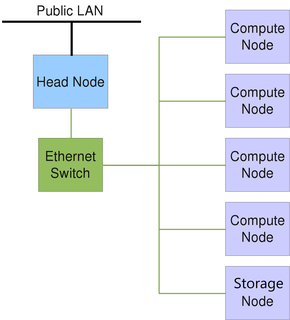
\includegraphics[width=.65\textwidth]{figures/HPC_cluster.png}
\centering
\caption{System Architecture of Cal Poly HPC Cluster\cite{hpc}}
\label{fig:hpccluser}
\end{figure}

\indent The Aerospace department at Cal Poly, SLO owns a server that is available to Aerospace students and faculty. It is referred to as Bishop High Performing Cluster\cite{hpc}. It includes a workload manager so that each user only needs to submit their jobs and they are separated through the different nodes on the cluster. The cluster allows each full user 48 cores and 64 GB of Ram\cite{hpc}. This is critical to SINATRA. Through the parallelization the simulation can be run in parallel on the server. Not only does Bishop have quick processors, but it also has the 48 cores that the simulation can be broken up between. This enables the execution time of a large simulation to be cut down \ref{tab:Timing} by significant amounts. This server also allows users to run simulations off of their local machines, which allows them to use them for everyday tasks. It also allows scheduling of multiple simulations ,therefore, large analysis tasks can be completed without human interface. SINATRA has been made with the Bishop cluster in mind and is able to be used with the cluster. \par




\indent Another simple process to reduce the execution time is during the linking phase. After the particles are created, they must be associated with the cells that they are in. To do this it requires a nested for loop  through all particles inside all cells. This is a very slow process. A few time reduction techniques have been implemented by the author, however, there is a simpler solution. There is an option in SINATRA to seed particles in a uniformly random way \cite{Galvez2018a}. This method creates the same number of particles in each cell but randomly distributes them within the cell. Now this linking process can be removed completely and the execution time reduces significantly. This has been implemented by the author. \par

\begin{table}
\label{tab:Timing}
\caption{Execution Time Comparisons}
\vspace{0.3cm}
\begin{center}
\begin{tabular}{|l|l|l|l|}
\hline
                             & First Iteration & Timestep Average & Total Time     \\ \hline
Parallel and No Linking & 9 sec           & 10 sec           & 1 min, 38 sec  \\ \hline
Serial and No Linking   & 3 min, 23 sec   & 3 min, 23 sec    & 33 min, 50 sec \\ \hline
Serial and Linking      & 15 min, 1 sec   &  3 min, 58 sec   &   50 min, 47 sec             \\ \hline
\end{tabular}
\end{center}
\end{table}

\indent A simple timing comparison was completed to examine the effectiveness of two execution time reduction methods. A collision-less simulation with all diffuse walls was run on the HPC server. The simulation used 32768 Cells, 5e19 real to simulated particles, 1e26 number density which gives 2 million simulation particles in the domain, 10 time steps of 1e-8 seconds each. As seen in Table \ref{tab:Timing}, including these optimization techniques has changed the simulation time drastically. By removing the linking process we were able to save a large amount of time during the set up\footnote{There is a slight difference in the iteration time for the linking and no linking runs because the no linking run did not use the uniform initialization because uniform initialization has has the linking section bypassed in the current version.}. Also, by adding the simple parallelization we were able to reduce the simulation time by 95\%. These two techniques combined make an appreciable difference in the execution time. They allow more complicated simulations to be run within the same amount of computation time. This allows the user to run longer simulations or multiple in order to increase confidence in the accuracy of the solution, as well as reduce the variance caused by the randomness in a DSMC simulation. \par

\indent Finally, an important tool for execution time analysis is debugging and profiling. It is important while developing software to have the ability to debug the code to see exactly what it is doing. This is usually achieved through the IDE; however, in an effort to make SINATRA IDE independent, the code has built in a method which allows the GNU Project Debugger to be used on the code\footnote{GDB: The GNU Project Debugger - \url{https://www.gnu.org/software/gdb/}}. This is a command line interface for g++ compiled executables. It is a legacy debugger that is well documented and is included in most installations of the g++ compiler. Using gdb on SINATRA allowed the author to solve problems within various improvements including removing linking and adding parallelized code. Secondly, a profiler allows the user to view exactly how often each line of code is run, how long it takes to run, and the sub processes, which contributes to that execution time. This is a strong way to identify simple coding bottlenecks and optimizing the coding time. The author has set up the compiling and code base in order to fit with the profilier Very Sleepy\textsuperscript{TM}\footnote{Very Sleepy documentation - \url{http://www.codersnotes.com/sleepy/}}. This is a light and simple profilier which shows each line of the source code and the timing involved. By setting up SINATRA to be largely universally compatible it allowed these developing tools to push SINATRA towards an industry standard level. \par


% Cite processer information
% Cite DSMC paralization papers

